\chapter{Convolutional Neural Networks (CNN)}

In Convolutional Neural Networks, the goal is to provide an image as an input and generate an output that determines the probability of the image belonging to a certain class. This chapter discusses the fundamentals of CNN as well as its various layers, i.e the Convolutional Layer, the Pooling Layer and the Fully Connected Layer.
\section{Introduction to \acrlong{cnn}}

Artificial Intelligence has contributed in a monumental manner to bridge the gap between humans and computer abilities. To make great things possible, researchers work on various facets of the area, the domain of Computer Vision being one of several such fields. The goal for this field is to allow machines to view the world as humans do, interpret it in a similar way and even use information for a variety of tasks, such as recognition of images and videos, reconstruction of media, recommendation systems, processing of natural languages, and so on. With time, the advances in Computer Vision with Deep Learning have been developed and refined, predominantly through a specific algorithm, a Convolutional Neural Network.

A Convolutional Neural Network (ConvNet/\acrshort{cnn}) is a deep learning algorithm that can take an input image, assign significance to various aspects/objects in the image and be able to distinguish one from the other. In comparison to other classification algorithms, the pre--processing required in a CNN is much lower. In \acrshort{cnn}, filters are not hand-engineered -- with enough training, they have the ability to learn these filters. 

The architecture of Convolutional Neural Networks differs from that of regular Neural Networks. In case of regular Neural Networks, an  is transformed by passing it through multiple hidden layers where each layer consists of a set of neurons and is entirely connected to all neurons in the layer before, following which there is a final fully-connected layer — the output layer — that represents the predictions. There is a slight difference in case of Convolutional Neural Networks. Here, the layers are organised in 3 dimensions: width, height and depth. Further, the neurons in one layer do not connect to all the neurons in the next layer but only to a small region of it. Ultimately, the final output will be reduced to a single vector of probability scores, organized along the depth dimension.
\section{Working of \acrlong{cnn}}
A \acrshort{cnn} has several layers for processing an image which are discussed below.
\subsection{Convolution Layer}
This is the first layer to extract features from an input image. An image is nothing but a matrix of pixel values. Convolution preserves the relationship between pixels by learning image features using small squares of input data. It is a mathematical operation that takes two inputs such as image matrix and a filter or kernel to produce a feature map. Convolution is executed by sliding the filter over the input. At every location, a matrix multiplication is performed between the image matrix and the filter matrix and the result is summed onto the feature map as shown in figures \ref{fig:imagemat} and \ref{fig:outputmat}. 

% \ref{fig:object} 
\begin{figure}[H]
\centering
	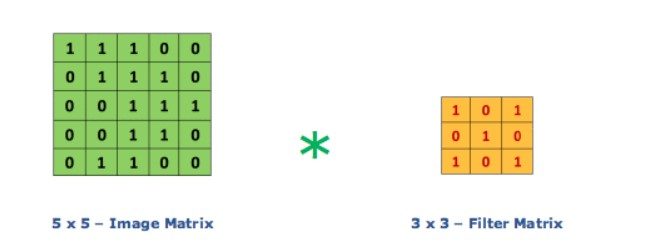
\includegraphics[scale=1]{Chapter2/img_mat_mul_kernel_filter_matrix.jpg}	
	\caption{Image matrix multiplied with kernel or filter matrix}
	\label{fig:imagemat}
\end{figure}
\begin{figure}[H]
\centering
	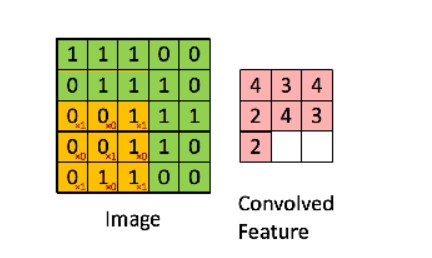
\includegraphics[scale=1]{Chapter2/output_mat.jpg}	
	\caption{Output matrix}
	\label{fig:outputmat}
\end{figure}
% INSERT IMGMATMUL AND OUTPUTMAT IMAGES HERE. 

Operations such as edge detection, blur and sharpen can be achieved by convolution of an image with different filters.


\subsection{Pooling Layer}
When the images are too large, pooling layers can reduce the number of parameters. Spatial pooling, also called subsampling or downsampling, reduces the dimensionality of each map but retains important information. Spatial pooling can be of several types:
\begin{enumerate}
    \item Max Pooling
    \item Average Pooling
    \item Sum Pooling
\end{enumerate}
Max Pooling returns the maximum value from the portion of the image covered by the kernel. Average Pooling returns the average of all the values from the portion of the image covered by the Kernel. Sum of all elements in the feature map is called Sum Pooling.

\begin{figure}[H]
\centering
	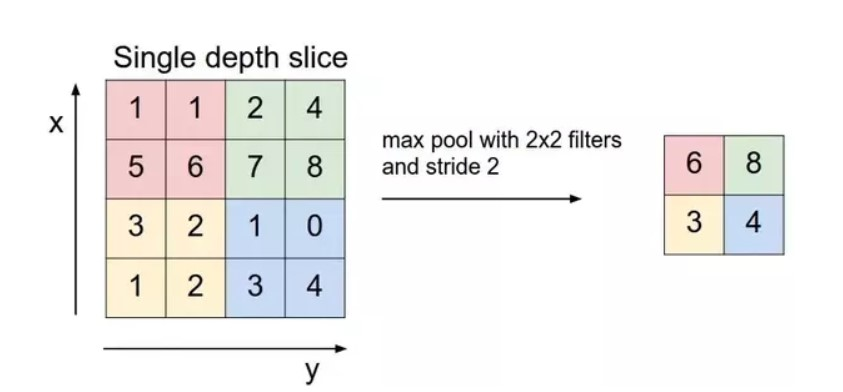
\includegraphics[scale=1]{Chapter2/max_pooling.jpg}	
	\caption{Max Pooling}
	\label{fig:maxpool}
\end{figure}
% INSERT MAX POOLING IMAGE HERE.

\subsection{Fully Connected Layer}
The input to the fully connected layer is the output from the final Pooling or Convolutional Layer, which is flattened (unroll the output of final (and any) Pooling and Convolutional Layer, which is a 3-dimensional matrix, values into a vector) and then fed into the fully connected layer.

\begin{figure}[H]
\centering
	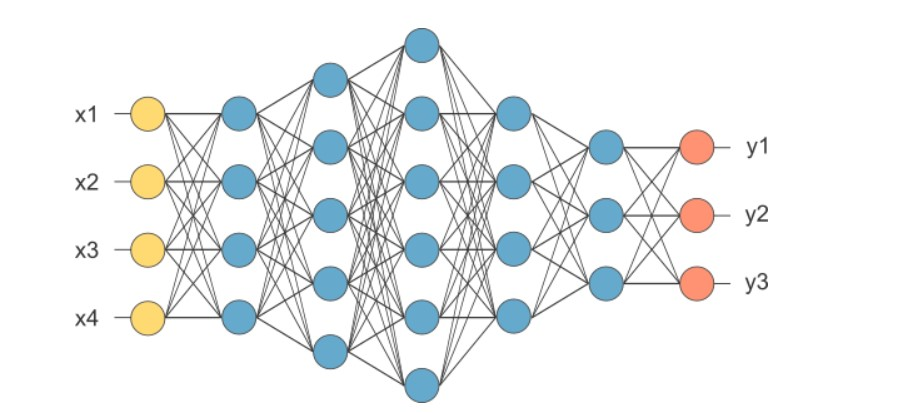
\includegraphics[scale=1]{Chapter2/after_pooling_layer_flattened_as_FC_layer.jpg}	
	\caption{After pooling layer, flattened as FC layer}
	\label{fig:after_pooling}
\end{figure}
% INSERT AFTERPOOLINGFLATTENED..FC IMAGE HERE.

In the above diagram, the feature map matrix will be converted as vector (x1, x2, x3, ...). With the Fully Connected Layers, we combine these features together to create a model. Finally, we have an activation function such as softmax or sigmoid to classify the outputs as  car, truck, cat, dog, etc.

\section{Other parameters associated with \acrshort{cnn} layers}

\subsection{Stride} 
It is the number of pixels shifts over the input matrix. We move the filter 1 pixel at a time when the stride is 1. We move the filter 2 pixels at a time when the stride is 2 and so on. Figure \ref{fig:stride} shows convolution would work with a stride of 2.

\begin{figure}[H]
\centering
	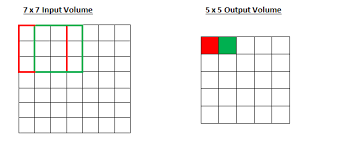
\includegraphics[scale=1]{Chapter2/stride.png}
	\caption{Stride}
	\label{fig:stride}
\end{figure}
% INSERT STRIDE IMAGE HERE.

\subsection{Padding}
There are times when the filter does not perfectly fit the input image. In such cases, there are two options:
\begin{enumerate}
    \item Pad the picture with zeros (zero-padding) so that it fits
    \item Drop the part of the image where the filter did not fit. This is called valid padding which keeps only valid part of the image.
\end{enumerate}

\subsection{Non Linear Activation function}
Activation functions are mathematical equations that determine the output of a neural network. The function is attached to each neuron in the network, and determines whether it should be activated (“fired”) or not, based on whether each neuron's input is relevant for the model's prediction. An example for activation function is ReLU (Rectified Linear Unit). ReLU is a non linear activation function defined as ƒ(x) $=$ max(0,x). It will output the input directly if it is positive, otherwise, it will output zero. It has become the default activation function for many types of neural networks since the problem of having negative weights can be avoided as negative values will be scaled to 0.

\begin{figure}[H]
\centering
	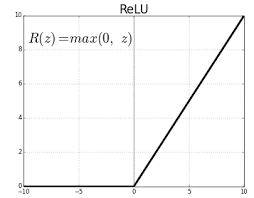
\includegraphics[scale=1]{Chapter2/relu.png}	
	\caption{ReLU activation Function}
	\label{fig:relu}
\end{figure}
% INSERT RELU IMAGE HERE.



% \section{Summary}
In summary, the CNN architecture is as follows. The input image is provided to the convolution layer. Parameters are chosen, filters with strides are applied along with padding, if required. Convolution on the image is performed and a non linear activation is applied to the matrix. Pooling is performed to reduce image dimension. The output of this stage is flattened and fed into a fully connected layer (FC Layer). This layer outputs the class to which the input image belongs.
\begin{figure}[H]
\centering
	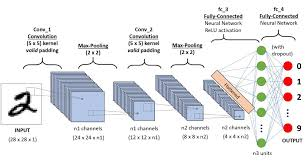
\includegraphics[scale=1.25]{Chapter2/cnn.jpeg}	
	\caption{CNN architecture}
	\label{fig:CNN}
\end{figure}
% INSERT COMPLETE CNN ARCHITECTURE IMAGE HERE.
